\documentclass{article}
\usepackage[margin=0.6in]{geometry}
\usepackage[utf8]{inputenc}
\usepackage{physics}
\usepackage{graphicx}
\usepackage{siunitx}
\usepackage{amsmath}
\usepackage{amssymb}
\usepackage[dvipsnames]{xcolor}
\usepackage[numbers,sort&compress]{natbib}
\usepackage{bm}
\usepackage{url}
\usepackage{hyperref}
\usepackage{parskip}
\usepackage{lineno}
\usepackage{float}
\linenumbers

\setlength\parindent{0pt}
\renewcommand{\baselinestretch}{1.5}

\usepackage{authblk}

\title{Optimal time-dependent deployments of climate control technologies}
\author[1,2]{Henri F. Drake\textsuperscript{*}}
\author[1]{Ron Rivest}
\author[1]{Alan Edelman}
\author[1]{John Deutch}
\affil[1]{Massachusetts Institute of Technology, Cambridge, MA, USA}
\affil[2]{Woods Hole Oceanographic Institution, Woods Hole, MA, USA}

\date{}             %% if you don't need date to appear
\setcounter{Maxaffil}{0}
\renewcommand\Affilfont{\itshape\small}

\begin{document}
\maketitle

\section{Model formulation}

\subsection{CO$_{2}$ concentrations: baseline emissions, emissions reductions, and negative emissions}

We assume a baseline emissions scenario which has emissions constant until 2060 and emissions decreasing linearly to zero in 2100 (Figure \ref{fig-configuration}a):
\begin{equation}
  q(t)=\begin{cases}
        5
        & \text{for $2020 \leq t < 2060$}\\
        5 (1 - \frac{t-t_{0}}{40})
        & \text{for $2060 \leq t < 2100$}\\
        0
        & \text{for  $2100 \leq t$}
       \end{cases} \quad\quad \text{ ppm/year}.
\end{equation}

CO$_{2}$ concentrations start at $c_{0}(t_{0}) = \SI{415}{ppm}$ in $t_{0}=2020$ and increase according to the emissions scenario $q(t)$, emissions reductions, and negative emissions. The baseline concentrations are simply $c_{0}(t) = c_{0}(t_{0}) + \int_{t'=t_{0}}^{t} q(t') \text{ d}t'$ (Figure \ref{fig-initial-guess}a). \textcolor{BlueViolet}{[Note: we currently assume all emitted CO$_{2}$ remains indefinitely in the atmosphere, ignoring the roughly 50\% of emissions that are in actually taken up by the ocean and biosphere.]} Emissions reductions are parameterized by the fractional reduction of yearly emissions $\phi(t) \in [0,1]$ such that the annual emissions become $q(1-\phi(t))$. Negative emissions are parameterized by the fraction $\varphi(t) \in [0,1]$ of the baseline emissions $q(t_{0}) = \SI{5}{ppm/year}$ in 2020 that are sequestered from the atmosphere in a given year (either by direct air capture, afforestation, or otherwise). The CO$_{2}$ concentrations in a given year are thus given by:
\begin{equation}
    c_{\phi, \varphi}(t) = c_{0}(t_{0}) + \int_{t'=t_{0}}^{t} q(t')(1-\varphi(t')) - q(t_{0}) \phi(t') \text{ d}t'.\label{eq-CO2-conc}
\end{equation}

\begin{figure}[htb!]
\noindent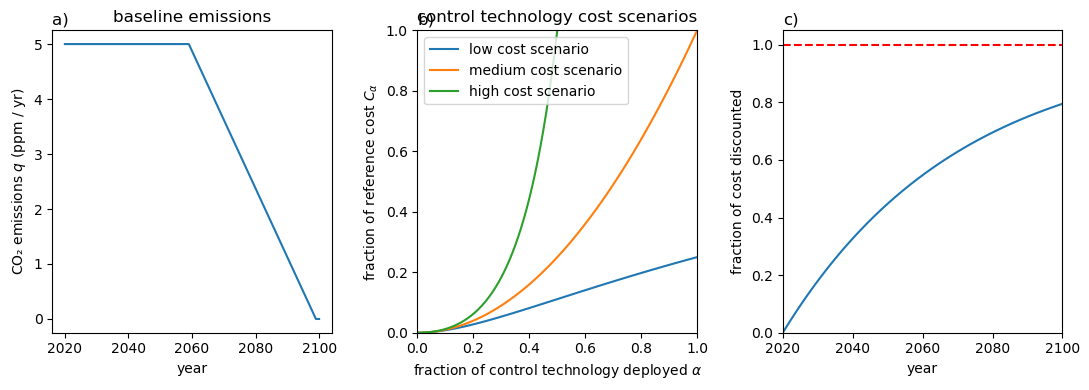
\includegraphics[width=1.0\textwidth]{figures/model_configuration.png}
\centering
\caption{(a) Idealized no-policy baseline emissions scenario. (b) Three different idealized functions for the cost scaling of climate control technologies. (c) The fraction of cost discounted by year under a 2\% utility discount rate.}
\label{fig-configuration}
\end{figure}

\subsection{Temperature response}
The linearized energy balance model underlying the model for the temperature response is:
\begin{equation}
    c_{f} \dv{T}{t} = -BT + F(t),
\end{equation}
where $c_{f}$ is the thermal heat capacity of the climate system, $B$ is the sensitivity parameter, $T$ is the temperature anomaly relative to a preindustrial mean (1850 to 1900), and $F(t)$ is an anthropogenic CO$_{2}$ forcing. We assume the thermal heat capacity of the climate system is sufficiently small such that $T(t)=F(t)/B$ at all times. \textcolor{BlueViolet}{[This is not a good assumption but is straight-forward and yields a fine first approximation; an improved model would include both the thermal heat capacity of the upper ocean and a second box for transfer to the high-capacity deep ocean.]} We determine the sensitivity parameter $B$ by tuning it to the best-guess estimate of the equilibrium climate sensitivity $T_{\text{ECS}} = F_{2\times}/B = \SI{3}{\celsius}$. Since $B = F_{2\times}/T_{\text{ECS}} = F(t)/T(t)$, we have $T(t) = T_{\text{ECS}} \frac{F(t)}{F_{2\times}}$. The greenhouse gas forcing due to CO$_{2}$ is well known to be a logarithmic function of concentration, $F(t)-F(t_{0}) = b \log(\frac{c(t)}{c(t_{0})})$.

The baseline temperature response to the baseline CO$_{2}$ concentrations is 
\begin{equation}
    T_{0}(t) = \frac{T_{\text{ECS}}}{\log(2)} \log(\frac{c_{0}(t)}{c_{0}(t_{0})}) = \epsilon \log(\frac{c_{0}(t)}{c_{0}(t_{0})}),
\end{equation}
where $\epsilon \equiv T_{\text{ECS}} / \log(2)$ is the transient warming parameter, while for the CO$_{2}$ concentration scenario $c_{\phi,\varphi}(t)$ it is given by
\begin{equation}
    T_{\phi,\varphi}(t) = \frac{T_{\text{ECS}}}{\log(2)} \log(\frac{c_{\phi,\varphi}(t)}{c_{0}(t_{0})}) = \epsilon \log(\frac{c_{\phi,\varphi}(t)}{c_{0}(t_{0})}).
\end{equation}


The temperature response can be further modified by solar radiation management or solar geongineering, which is parameterized by reducing the emissions-controlled temperature response $T_{\phi,\varphi}$ by a fraction $\lambda(t) \in [0,1]$, such that the controlled temperature response is given by:
\begin{equation}
    T_{\phi, \varphi, \lambda} = \epsilon \log(\frac{c_{\phi,\varphi}(t)}{c_{0}(t_{0})})(1 - \lambda(t)).
\end{equation}

\subsection{Climate damages}

Yearly climate damages are assumed to be of the quadratic form $D(t) = \beta T(t)^{2}$, such that successive temperature increases are increasingly damaging. The baseline climate damages are thus
\begin{equation}
    D_{0}(t) = \beta T_{0}(t)^{2}.
\end{equation}
Adaptation to climate change impacts (e.g. building sea walls, installing air conditioning units, planting climate-resilient crops) is parameterized by reducing yearly damages by a fraction $\chi(t) \in [0,1]$, such that the total controlled damages are:
\begin{equation}
    D_{\phi, \varphi, \lambda, \chi} = \beta \; (T_{\phi, \varphi, \lambda}(t))^{2} \; (1-\chi(t)).
\end{equation}

\subsection{Control costs}

The yearly cost of climate control technologies are given by
\begin{equation}
    C(t) = \sum_{\alpha \in \mathcal{A}} C_{\alpha} f(\alpha(t)),
\end{equation}
where $\mathcal{A} = \{ \phi, \varphi, \lambda, \chi \}$ is the set of climate control technologies considered here, $C_{\alpha}$ is reference cost of each climate control technology, and $f(\alpha)$ is a function that determines how the deployment cost increases as a function of fractional deployment. Here, we will focus on the medium deployment cost scenario $f_{\text{med}}(\alpha) = \alpha^{2}$, which has the following convenient properties: 
\begin{itemize}
    \item $\left. \dv{f}{\alpha}\right|_{\alpha=0} = 0$ (initial deployment is effectively free),
    \item $f(1) = 1$ (full deployment costs $C_{\alpha}$), and
    \item $\dv[2]{f}{\alpha} > 0$ (deployment gets progressively more and more expensive).
\end{itemize}
We also leave open the possibility of low cost $f_{\text{low}} = \left( \frac{\alpha}{1+\alpha} \right)^{2}$ and high cost $f_{\text{high}} = \left( \frac{\alpha}{1-\alpha} \right)^{2}$ deployment scenarios (Figure \ref{fig-configuration}b) but do not explore them further here. 

\subsection{Total costs and discounting}

The total yearly costs of climate change are the sum of the (uncontrolled or controlled) climate damages and the costs of control technologies. A common economic assumption is that society discounts future costs relative to present costs by a multiplicative factor $(1 + \rho)^{-(t-t_{0})}$ (Figure \ref{fig-configuration}c), determined by the utility discount rate $\rho$. The discounted total cost (in dollars) of climate change from $t_{0} = 2020$ to $t_{f} = 2100$ is thus given by:
\begin{equation}
    \mathcal{T} =
    \int_{t'=t_{0}}^{t_{f}}
    (C(t') + D_{\mathcal{A}}(t')) (1 + \rho)^{-(t'-t_{0})} \text{ d}t'
\end{equation}

The economic model parameters used in the following example are given in the table below.

\begin{center}
 \begin{tabular}{|c || c | c | c | c | c | c | c||}
 \hline
 Experiment &
 Global World Product (GWP) &
 $\beta$ &
 $\rho$ &
 $C_{\phi}$ &
 $C_{\varphi}$ &
 $C_{\lambda}$ &
 $C_{\chi}$ \\
 Name &
 [\si{\$/yr}] &
 [\si{GWP/\celsius^{2}}] &
 &
 [\si{GWP}] &
 [\si{GWP}] &
 [\si{GWP}] &
 [\si{GWP}] \\[0.5ex]
 \hline\hline
 Example &
 100 &
 0.01 &
 0.03 &
 0.05 &
 0.05 &
 0.1 &
 0.15 \\ 
 \hline
\end{tabular}
\end{center}

\subsection{Optimization Method}

As a crude first attempt at optimizing the control parameters $\mathcal{A} = \{\phi, \varphi, \lambda, \chi\}$, we use a simple gradient descent algorithm (with momentum) to final the minimum of the modified cost function

\begin{equation}
    \mathcal{T}_{M} =
    \int_{t'=t_{0}}^{t_{f}}
    (C(t') + D_{\mathcal{A}}(t')) (1 + \rho)^{-(t'-t_{0})} \text{ d}t'
    + \tau \sum_{\alpha \in \mathcal{A}} \left( \sum_{t} \left(\pdv{\alpha}{t} \right)^{2} + \alpha(t_{0})^{2} \right),
\end{equation}
where $\tau = 200$ is large relative to $\mathcal{T}$ and the new terms are ad-hoc modifications that enforce additional constraints on the optimization: the first term in the sum effectively enforces continuity of the control parameters in time and the second term asserts that there is no deployment of climate control technologies in 2020, $\alpha(t_{0})=0$.

We begin the optimization algorithm with an arbitrary (but physically possible) initial guess, depicted in Figure \ref{fig-initial-guess}. In this initial scenario, all of the climate control parameters increase linearly with time from zero deployment in 2020 to varying levels of deployment in 2100 (Figure \ref{fig-initial-guess}a). As a result of aggressive emissions reductions and gradually increasing deployment of negative emissions technologies, CO$_{2}$ concentrations peak at $c_{\phi, \varphi} = \SI{550}{ppm}$ in around 2070 and decrease thereafter. As a result of these controls on carbon and a small deployment of solar geoengineering, peak at $T_{\lambda, \phi, \varphi} = \SI{2.4}{\celsius}$, temporarily overshooting the $\SI{2}{\celsius}$ before cooling to below $\SI{2}{\celsius}$ by 2095. By chance, we have chosen an initial guess for which the total (controlled) costs of climate change are substantially smaller than the uncontrolled damages. This is not guaranteed to be the case – naive deployment of climate control technologies can lead to total costs which exceed the uncontrolled damages! This is increasingly likely to occur if the costs of controls are higher than assumed here (e.g. either be increasing $C_{\alpha}$ or by assuming deployment costs follow $f_{\text{high}}$).

\begin{figure}[htb!]
\noindent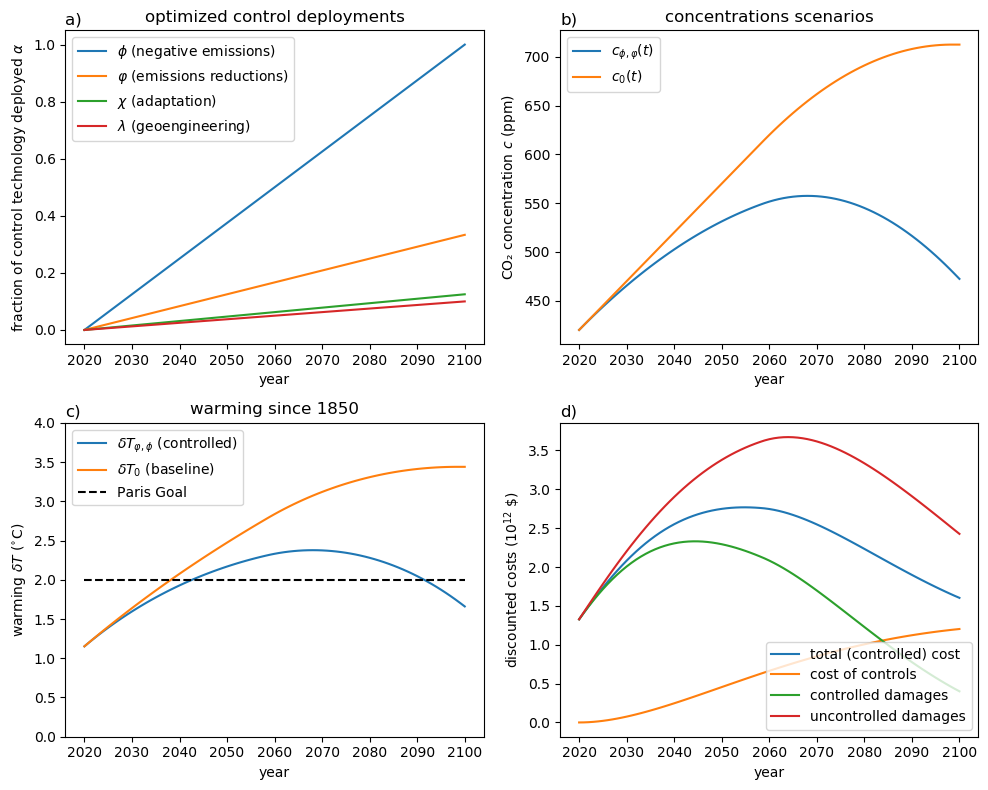
\includegraphics[width=1.0\textwidth]{figures/model_trajectories_initial_guess.png}
\centering
\caption{(a) Idealized no-policy baseline emissions scenario. (b) Three different idealized functions for the cost scaling of climate control technologies. (c) The fraction of cost discounted by year under a 2\% utility discount rate.}
\label{fig-initial-guess}
\end{figure}

\subsection{Results}
The results of the optimization process are shown in Figure \ref{fig-optimized}. In contrast to our initial guesses of deployment trajectories, the optimal solution includes rapid deployment of emissions reductions and negative emissions (Figure \ref{fig-optimized}a). Emissions reductions are phased out starting around 2060, as the baseline emissions begin decreasing and fractional emissions reductions thus become less effective at decreasing climate damages. Negative emissions are similarly phased out, though not as rapidly as emissions reductions because their effectiveness depends only on the baseline emissions at 2020, not the simultaneous baseline emissions. As a result of these controls on carbon, concentrations increase at roughly half the rate of the baseline scenario before plateauing at \SI{550}{ppm} around 2080 (Figure \ref{fig-optimized}b). Adaptation and geoengineering are gradually deployed, replacing negative emissions and emissions reductions in the second half of the century (Figure \ref{fig-optimized}a).

\begin{figure}[htb!]
\noindent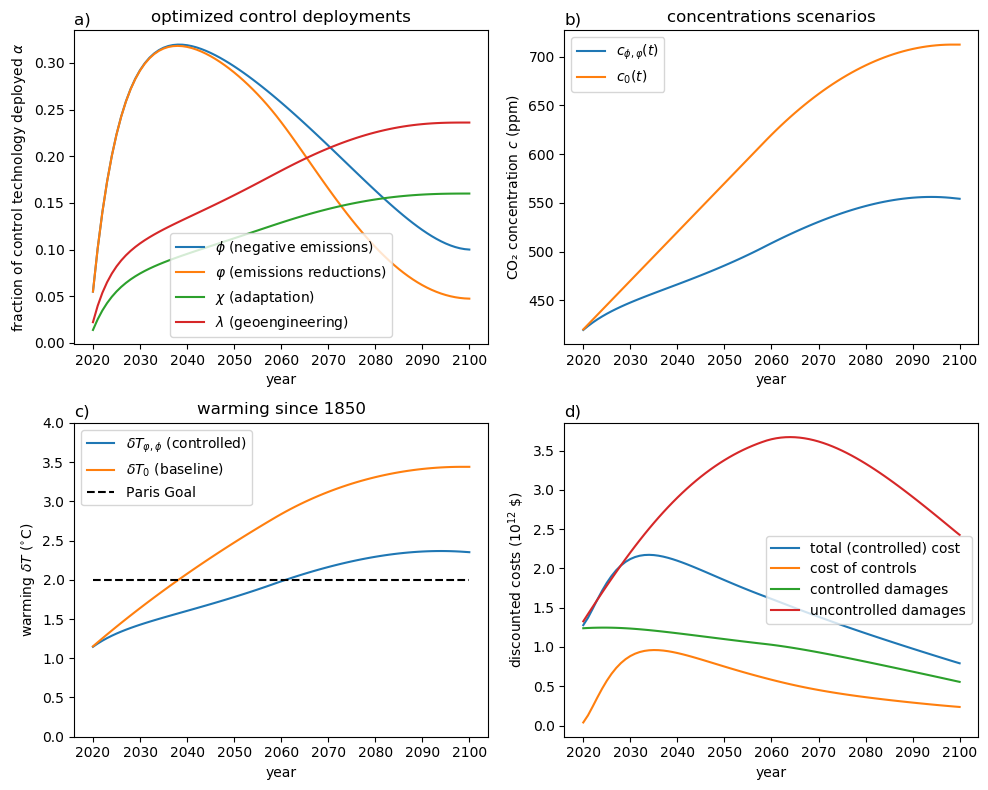
\includegraphics[width=1.0\textwidth]{figures/model_trajectories_optimized.png}
\centering
\caption{(a) Idealized no-policy baseline emissions scenario. (b) Three different idealized functions for the cost scaling of climate control technologies. (c) The fraction of cost discounted by year under a 2\% utility discount rate.}
\label{fig-optimized}
\end{figure}

Temperatures increase gradually before plateauing at about \SI{2.4}{\celsius} around 2080 (Figure \ref{fig-optimized}c). While the temperature anomaly reaches the same maximum of $T_{\phi, \varphi, \lambda} = \SI{2.4}{\celsius}$ in the optimal solution as in the initial guess (Figure \ref{fig-optimized}c and Figure \ref{fig-initial-guess}c), the optimal solution reaches its maximum about 25 years later, resulting in dramatically less yearly controlled climate damages after discounting (green lines in Figure \ref{fig-optimized}d and Figure \ref{fig-initial-guess}d). While the optimal solution results in larger total yearly discounted costs than both the uncontrolled damages and the initial guess, the total yearly costs after 2030 are substantially less than both the initial guess and the uncontrolled damages. The total discounted cost from 2020 to 2100 is the integral under the yearly cost curves in Figures \ref{fig-initial-guess}d and \ref{fig-optimized}d. The total discounted cost in the optimal solution is smaller than both the the uncontrolled cost and the cost of the initial guess by about a factor of two.

\section{Next steps}

\subsection{Improved optimization algorithm}

I am new to optimization and did the simplest thing I could think of. The primary downsides of this approach are: 1) it assumes we reach the first minimum we reach from our initial guess is the global minimum (perhaps this is a fine assumption for this relatively small number of dimensions and smooth cost function); 2) it is slow (~20 seconds per simulation), making large ensemble simulations (e.g. stochastic or monte carlo) intractable for the time being; 3) the imposed constraints are ad-hoc and somewhat arbitrary (is there a better way of imposing continutiy and initial / boundary conditions?).

\subsection{Imposing a budget constraint}

I have taken the approach of minimizing the total cost of climate change, including both the cost due to (controlled or uncontrolled) climate damages and the cost of deploying climate control technologies. Jon Deutch's approach was somewhat different: he prescribed a total budget and aimed to minimize the controlled climate damages within the prescribed budget. I think both are equally interesting.

\subsection{Transient heat and carbon uptake}
Anthropogenically-emitted carbon and heat trapped by anthropogenically-emitted carbon do not stay in the atmosphere once emitted. Over the last hundred of so years, $90\%$ of anthropogenic heat and $30\%$ of anthrogenic carbon have been absorbed by the ocean, by exchange with atmosphere at the sea surface and subsequent turbulent transfer into the deep ocean. \textcolor{BlueViolet}{[About $20\%$ of the carbon was also absorbed by the biosphere, but for our purposes we can probably ignore this process).]}

We are effectively ignoring both of these important transient uptake processes and could incorporate both with simple two-box models.

\subsection{Monte Carlo simulations}

Our model currently doesn't take into account any uncertainty or stochastic effects. One could imagine myriad additional complexities, but some a physical climate scientists' perspective, one of the most interesting additions would be uncertainty in the equilibrium climate sensitivity. The consensus view is that the equilibrium climate sensitivity is between about $\SI{1.5}{\celsius}$ and $\SI{4.5}{\celsius}$. Given the non-linearities in the climate damage and deployment cost functions, the projection of uncertainties in the equilibrium climate sensitivity onto the optimal controls may be interesting.

%\bibliographystyle{naturemag}
%\bibliography{climate-model-performance.bib,manual_refs.bib}

\end{document}